\documentclass[a4paper,11pt]{ltjsarticle}

\usepackage{luatexja}
\usepackage{geometry}
\geometry{margin=25mm}

\usepackage{array}
\usepackage{longtable}
\usepackage[table]{xcolor}
\usepackage{booktabs}

\usepackage{enumitem}

\usepackage{hyperref}

\usepackage{titlesec}
\titleformat{\section}{\large\bfseries}{\thesection.}{0.5em}{}

\usepackage{listings}
\lstset{
  basicstyle=\ttfamily\small,
  frame=single,
  breaklines=true,
  numbers=left,
  numberstyle=\tiny\color{gray},
  keepspaces=true,
  showstringspaces=false,
  columns=fullflexible,
  tabsize=2,
}

\usepackage{tikz}
\usetikzlibrary{shapes.geometric, arrows.meta, positioning, calc, fit}

\usepackage{graphicx}

\usepackage{float}

\definecolor{ganttCell}{HTML}{4FC3D0}
\definecolor{ganttEarly}{HTML}{FFB74D}

\providecommand{\％}{\%}

\setlength{\parindent}{0pt}
\setlist[itemize]{leftmargin=2em}

\setlength{\emergencystretch}{6em}

\begin{document}

\begin{center}
    {\LARGE \textbf{第10回事前課題}}\\[0.4em]
    {\large 作業ログ（第9週末）}\\[1em]
\end{center}

\begin{tabular}{|p{4cm}|p{10cm}|}
\hline
報告者 & 櫛濱 和輝 (25G1046)\\
\hline
報告日 & 2026年7月1日\\
\hline
チーム & チーム9\\
\hline
プロジェクト名 & 赤外線通信で歌うカエル\\
\hline
担当パート & 親機 hack\_oya\_kai2.ino のテンポ制御 UI 改善（BPM 可変抵抗化），子機 hack-koP2.ino の楽譜送出ロジック整備，Processing 側 hackko.pde のピアノ音色リアル化（倍音構造/ADSR 調整），および親機の退場予約ロジック整備\\
\hline
本来の今週の位置づけ & 第9週末（6/30）．計画書 v1.1（2026/6/19版）のガント上，第9週は 510:結合テストの継続期間．前回個人作業ログ（6/24）で挙げた次回計画のうち，MOP3 テンポ変更追従に関連する BPM 制御の改善と，MOP4 音色再現性に関連するピアノ音のリアル化を今週引き取り対応\\
\hline
報告対象 & 前回個人作業ログ（6/24）以降に実施した親機テンポ制御の UI 改善とピアノ音のリアル化．具体的には親機 hack\_oya\_kai2.ino の BPM 変更手段を D9 デジタルボタン（固定段階切替）から A5 ポテンショメータ（10k$\Omega$ シングルターン可変抵抗器，60--150 BPM 連続調整）への置換，退場予約を子機の現ループ末尾（SCORE\_TICKS=32）までアライメントする改善，Processing hackko.pde のピアノ音色における倍音構造の再調整と ADSR エンベロープの改善\\
\hline
作業時間 & 計8時間\\
\hline
\end{tabular}

\vspace{1em}

%=====================================================
\section{進捗サマリー}\label{sec:summary}

\begin{itemize}
    \item 現在地：第9週末（6/30）．510:結合テストの継続期間．前回作業ログ（6/24）で 4 子機の輪唱実機稼働まで完了しており，今週は演奏時の操作性向上と音色品質の改善に注力した
    \item 親機 hack\_oya\_kai2.ino の BPM 制御改善：
    \begin{itemize}
        \item BPM 変更手段を D9 ボタン（押すたびに固定値を切り替える方式）から A5 ポテンショメータ（uxcell 10k$\Omega$ シングルターン可変抵抗器）に置換した．指でノブを回すだけで 60--150 BPM の範囲を連続的に調整でき，演奏中でもリアルタイムにテンポが変わる
        \item \texttt{handleTempoPot()} 関数で 50ms 間隔にアナログ値を読み取り，指数移動平均（\texttt{smoothedPotRaw = (smoothedPotRaw * 3 + raw) / 4}）でノイズを抑えた上で \texttt{map()} により BPM に変換する．tick 周期計算は毎ループ \texttt{tempoBpm} を参照しているため，ポテンショメータを回した瞬間から演奏テンポに反映される
        \item シリアルログの抑制として，BPM が 2 以上変化したときだけ \texttt{tempo=N} を出力する仕組みにした．微小な ADC 揺らぎでログが埋まる症状を防止
    \end{itemize}
    \item 退場予約ロジックの改善：
    \begin{itemize}
        \item 子機の退場予約を，直近の \texttt{QUANTIZE\_TICKS}（8 tick）境界ではなく，その子機が参加した時点（\texttt{joinedAtTick}）から数えて次の \texttt{SCORE\_TICKS}（32 tick＝楽譜1周分）境界にアライメントする方式に変更した．子機が演奏途中で突然切れるのではなく，現在のループを最後まで弾き切ってから抜けるようになった
    \end{itemize}
    \item ピアノ音のリアル化（hackko.pde）：
    \begin{itemize}
        \item \texttt{WavetableGenerator.gen10} の倍音構成パラメータを調整し，実際のピアノの倍音構造に近い振幅比（基音 1.0，第2倍音 0.6，第3倍音 0.35，第4倍音 0.2，第5倍音 0.1，第6倍音 0.05）を設定した．従来の単純な矩形波/正弦波ベースの音色と比べて厚みが出て，ピアノらしい音色に近づいた
        \item \texttt{PianoInstrument} クラスに 5Hz のビブラート（\texttt{Oscil} で周波数を微小変調）と \texttt{Line} による線形減衰エンベロープを実装し，アタック直後から自然に音量が減衰するピアノらしい発音特性を再現した
    \end{itemize}
    \item 全体進捗率：510:結合テストは前回の 4 子機輪唱実機稼働に加え，テンポ制御の連続可変化とピアノ音色の改善が完了．残課題は MOP1 演奏タイミング誤差と MOP2 赤外線通信成功率の定量計測，双子音処理の非ブロック化
    \item 主要成果：
    \begin{itemize}
        \item ポテンショメータによる BPM 連続調整で，演奏者が楽曲に合わせてテンポを直感的に操作できるようになった．ボタン式では 120/150 等の固定値しか選べなかったところが，任意の BPM に即座に合わせられる
        \item ピアノ音に倍音と減衰エンベロープを加えたことで，聴感上の音色品質が向上し MOP4 の達成に近づいた
        \item 退場予約のループ末尾アライメントにより，演奏途中で子機が突然抜ける不自然さが解消された
    \end{itemize}
\end{itemize}

%=====================================================
\section{ガントチャート}\label{sec:gantt}

第9週末時点では計画書 v1.1（2026/6/19版）から変更はないため，チーム全体/個人とも v1.1 のガントチャートのみを掲載する．着色セル（\colorbox{ganttCell}{\phantom{xx}}）は当該タスクの実施週を表す．

\renewcommand{\arraystretch}{1.3}

\begingroup
\setlength{\tabcolsep}{3pt}

\subsection{チーム全体ガントチャート}\label{sec:gantt-team}

\begin{longtable}{|p{6.2cm}|p{2.3cm}|c|c|c|c|c|c|}
\hline
\rowcolor[gray]{0.9}
第3層：活動タスク & 担当者 & 5週 & 6週 & 7週 & 8週 & 9週 & 10週 \\
\hline
110:ピアノ音の作成 & 櫛濱・久家 & \cellcolor{ganttCell} & & \cellcolor{ganttCell} & & & \\
\hline
120:arduinoとの通信用関数（ピアノ） & 櫛濱・久家 & \cellcolor{ganttCell} & & & & & \\
\hline
130:フルート音の作成 & 家田 & \cellcolor{ganttCell} & & & & & \\
\hline
140:arduinoとの通信用関数（フルート） & 家田 & \cellcolor{ganttCell} & & & & & \\
\hline
150:トランペット音の作成 & 木下 & \cellcolor{ganttCell} & & & & & \\
\hline
160:arduinoとの通信用関数（トランペット） & 木下 & \cellcolor{ganttCell} & & & & & \\
\hline
170:ドラム音の作成（キック） & 久家 & & \cellcolor{ganttCell} & & & & \\
\hline
171:ドラム音の作成（シンバル） & 久家 & & \cellcolor{ganttCell} & & & & \\
\hline
180:arduinoとの通信用関数（ドラム） & 久家 & & \cellcolor{ganttCell} & & & & \\
\hline
210:ピアノのプログラム & 櫛濱 & \cellcolor{ganttCell} & & & & & \\
\hline
220:フルートのプログラム & 家田 & \cellcolor{ganttCell} & & & & & \\
\hline
230:トランペットのプログラム & 木下 & \cellcolor{ganttCell} & & & & & \\
\hline
240:ドラムのプログラム & 久家 & & \cellcolor{ganttCell} & & & & \\
\hline
250:楽譜進行プログラム & 渡邊 & & \cellcolor{ganttCell} & \cellcolor{ganttCell} & \cellcolor{ganttCell} & & \\
\hline
310:赤外線管理プログラム & 家田・渡邊 & & \cellcolor{ganttCell} & \cellcolor{ganttCell} & \cellcolor{ganttCell} & & \\
\hline
320:テンポ管理プログラム & 渡邊 & & \cellcolor{ganttCell} & & & & \\
\hline
410:回路作成 & 手代木 & & \cellcolor{ganttCell} & & & & \\
\hline
420:LEDマトリクス作成 & 手代木 & & \cellcolor{ganttCell} & \cellcolor{ganttCell} & \cellcolor{ganttCell} & & \\
\hline
510:結合テスト & 全員 & & & & \cellcolor{ganttCell} & \cellcolor{ganttCell} & \cellcolor{ganttCell} \\
\hline
\end{longtable}

\endgroup

\subsection{個人ガントチャート（計画書 v1.1 から櫛濱担当分を抜粋）}\label{sec:gantt-personal}

\ref{sec:gantt-team} 節のチーム全体ガントから櫛濱担当分を抜き出した個人計画．第9週は 510:結合テストの継続期間．本週は親機の BPM 制御をポテンショメータに置換してテンポの連続可変化を実現し，ピアノ音の倍音構造/ADSR を調整して音色品質を改善した．

\begingroup
\setlength{\tabcolsep}{3pt}
\begin{longtable}{|p{0.9cm}|p{2.0cm}|p{5.2cm}|c|c|c|c|c|c|}
\hline
\rowcolor[gray]{0.9}
管理 & 第2層 & 第3層タスク & 5週 & 6週 & 7週 & 8週 & 9週 & 10週 \\
\hline
110 & 100 (Processing) & ピアノ音の作成 & \cellcolor{ganttCell} & & \cellcolor{ganttCell} & & & \\
\hline
120 & 100 (Processing) & arduinoとの通信用関数（ピアノ） & \cellcolor{ganttCell} & & & & & \\
\hline
170 & 100 (Processing) & ドラム音の作成（キック） & & \cellcolor{ganttCell} & & & & \\
\hline
210 & 200 (子機) & ピアノのプログラム & \cellcolor{ganttCell} & & & & & \\
\hline
510 & 500 (包括) & 結合テスト（全員） & & & & \cellcolor{ganttCell} & \cellcolor{ganttCell} & \cellcolor{ganttCell} \\
\hline
\end{longtable}
\endgroup

\subsection{今週の作業位置づけ}\label{sec:gantt-position}

\begin{itemize}
    \item 現在地は第9週末（6/30）．GC 上，第9週は 510:結合テストの継続期間．前回作業ログ（6/24）で 4 子機の輪唱実機稼働を完了しており，今週はテンポ制御の操作性と音色品質の改善に取り組んだ
    \item 親機 hack\_oya\_kai2.ino の BPM 制御を D9 デジタルボタン（固定段階切替）から A5 ポテンショメータ（10k$\Omega$ シングルターン可変抵抗器）に変更し，60--150 BPM の連続調整を可能にした．MOP3 テンポ変更追従の評価基盤として，ポテンショメータ操作が即座にテンポに反映されることを確認
    \item 退場予約を \texttt{QUANTIZE\_TICKS}（8 tick）境界から \texttt{SCORE\_TICKS}（32 tick＝楽譜1周）境界にアライメントするよう変更し，子機がループ途中で切れる不自然さを解消
    \item Processing hackko.pde のピアノ音色を，倍音構成パラメータの再調整とビブラート/線形減衰エンベロープの追加によりリアル化した．MOP4 音色再現性の達成に向けた取り組み
    \item 次週（第10週/最終週）は残る MOP1/MOP2 の定量計測と，双子音処理の非ブロック化，最終発表の準備を進める
\end{itemize}

%=====================================================
\section{作業ログ}\label{sec:worklog}

\renewcommand{\arraystretch}{1.4}

\begingroup
\setlength{\tabcolsep}{3pt}
\sloppy
{\footnotesize
\begin{longtable}{|p{2.6cm}|p{1.1cm}|p{1.3cm}|p{1.0cm}|p{0.9cm}|p{2.2cm}|p{4.5cm}|}
\hline
\rowcolor[gray]{0.9}
作業項目 & 開始日 & 予定完了日 & 状態 & 進捗率 & 依存関係・ブロッカー & コメント \\
\hline
hack\_oya\_kai2 の新規作成（退場予約トグル + LED 同期） & 6/25 & 6/26 & 完了 & 100\％ & hack-oya.ino ベース & hack-oya.ino をベースに，参加/退場のリアルタイムトグルを実装．ボタン押下ごとに未参加→参加予約→参加中→退場予約→退場の状態遷移をトグルで操作できる．A0--A3 LED は内部状態を XOR 論理で同期表示 \\
\hline
BPM 変更をポテンショメータ化（hack\_oya\_kai2） & 6/26 & 6/27 & 完了 & 100\％ & A5 アナログ入力 / 10k$\Omega$ ポテンショメータ & D9 ボタンによる固定段階切替から A5 ポテンショメータ（uxcell 10k$\Omega$ シングルターン）に置換．\texttt{handleTempoPot()} で 50ms 間隔に読み取り，指数移動平均で平滑化後 60--150 BPM にマッピング．演奏中にノブを回すだけでリアルタイムにテンポが変わる \\
\hline
退場予約のループ末尾アライメント & 6/27 & 6/27 & 完了 & 100\％ & \texttt{joinedAtTick} / \texttt{SCORE\_TICKS=32} & 退場予約の発火タイミングを \texttt{QUANTIZE\_TICKS}(8) 境界から \texttt{SCORE\_TICKS}(32) 境界に変更．\texttt{joinedAtTick} から経過 tick 数を割って次のループ末尾を算出し，子機が楽譜を最後まで弾き切ってから抜ける \\
\hline
ピアノ音のリアル化（hackko.pde） & 6/28 & 6/29 & 完了 & 100\％ & Minim \texttt{WavetableGenerator} / \texttt{PianoInstrument} & \texttt{gen10} の倍音振幅を 6 次まで設定（1.0, 0.6, 0.35, 0.2, 0.1, 0.05）し実ピアノの倍音構造に近づけた．\texttt{PianoInstrument} に 5Hz ビブラートと \texttt{Line} 減衰エンベロープを追加し，アタック直後から自然に減衰するピアノらしい発音特性を実現 \\
\hline
hack-koP2.ino の整備 & 6/29 & 6/30 & 完了 & 100\％ & hack-ko.ino ベース / hack\_oya\_kai2 プロトコル & hack\_oya\_kai2 の mask ベースプロトコルに対応した子機ファームを完成版ver1 として整備．\texttt{TOTAL\_TICKS} によるループ再生と双子音区間の送出を維持しつつ，親機側の新しいプロトコルに整合させた \\
\hline
\end{longtable}
}
\endgroup

%=====================================================
\section{評価事項}\label{sec:evaluation}

計画書 v1.1（2026/6/19版）の V\&V 計画のうち，今週の作業（BPM ポテンショメータ化/退場予約改善/ピアノ音リアル化）に対応する項目を整理する．

\subsection{対応する有効指標 MOE}\label{sec:moe}

\begin{longtable}{|p{1.2cm}|p{4cm}|p{8cm}|}
\hline
\rowcolor[gray]{0.9}
No. & MOE & 評価基準 \\
\hline
MOE1 & 違和感なく聞くことができる & 輪唱が聴衆にズレを感じさせることなく演奏できている．テンポ変更時も滑らかに追従する \\
\hline
MOE3 & 楽器音らしい音色である & Processing で合成した音が楽器音として聴衆に認識される \\
\hline
\end{longtable}

\subsection{対応する性能指標 MOP（計画書 v1.1）}\label{sec:mop}

\begin{longtable}{|p{1.2cm}|p{3.8cm}|p{8.8cm}|}
\hline
\rowcolor[gray]{0.9}
No. & 性能指標 & 目標値・評価基準 \\
\hline
MOP1 & 演奏タイミング誤差 & 各演奏側 Arduino 間の音符開始タイミングのズレが 30 ms 以内であること \\
\hline
MOP2 & 同期信号の受信成功率 & 指揮側から送信した赤外線信号を演奏側が正しく受信できる割合が 95\% 以上であること \\
\hline
MOP3 & テンポ変更への追従時間 & 指揮側がテンポを変更してから演奏側全台が新テンポに追従するまでの時間が 1 拍以内であること \\
\hline
MOP4 & 音色の再現性 & 倍音構造/ADSR の設定により，対応する楽器の音色として聴衆の過半数に評価されること \\
\hline
\end{longtable}

\subsection{今週の自己評価}\label{sec:selfeval}

\begingroup
\setlength{\tabcolsep}{3pt}
\sloppy
\begin{longtable}{|p{1.0cm}|p{2.8cm}|p{1.8cm}|p{8.7cm}|}
\hline
\rowcolor[gray]{0.9}
No. & 項目 & 達成状況 & 備考 \\
\hline
MOE1 & 違和感なく聞ける輪唱 & OK & 前回完了した 4 子機輪唱を維持．テンポ変更時も聴感上の破綻なし \\
\hline
MOE3 & 楽器音らしい音色 & 改善 & ピアノ音の倍音構造を 6 次まで設定し，ビブラートと減衰エンベロープを加えたことで聴感上の音色品質が向上 \\
\hline
MOP1 & 演奏タイミング誤差 & 暫定OK & 聴感では破綻なし．第10週に上方動画撮影+各子機付近の iPhone 録音+DAW 波形計測で定量評価予定（未実施） \\
\hline
MOP2 & 同期信号受信成功率 & 暫定OK & 4 子機同時受信は確認．95\% 目標との定量比較は未実施（第10週で対応） \\
\hline
MOP3 & テンポ変更追従時間 & OK & ポテンショメータを回した瞬間から \texttt{tempoBpm} が更新され，次の tick 周期計算に即反映される．追従遅延は 1 tick 以内（1 拍未満）であることを聴感で確認 \\
\hline
MOP4 & 音色の再現性 & 部分対応 & ピアノ音を倍音/ADSR で改善済み．聴衆過半数の評価はアンケート未実施 \\
\hline
\end{longtable}
\endgroup

\subsection{今後評価予定の項目（参考）}\label{sec:futureplan}

\begin{itemize}
    \item MOP1：演奏風景を上方から動画撮影しつつ，各子機の近くに iPhone を置いてマイクで同時録音する．収録した音声を DAW に取り込み，波形上で各子機の音符開始タイミングのズレを計測して 30ms 以内であることを確認（第10週，未実施）
    \item MOP2：4 子機を一定時間動かして送受信ログから成功率を算出（第10週）
    \item MOP4：音色認識テスト（聴衆過半数が各楽器と識別，アンケート実施予定）
    \item MOP5：歌詞/アニメーション同期遅延（LCD 担当の手代木範囲）
\end{itemize}

%=====================================================
\section{課題管理}\label{sec:issues}

\begingroup
\setlength{\tabcolsep}{3pt}
\sloppy
{\footnotesize
\begin{longtable}{|p{2.6cm}|p{3.2cm}|p{0.9cm}|p{0.9cm}|p{3.4cm}|p{1.3cm}|p{1.3cm}|}
\hline
\rowcolor[gray]{0.9}
課題 & 発生原因 & 影響度 & 優先度 & 対策 & 期限 & 状態 \\
\hline
双子音処理の \texttt{delay()} による IR 取りこぼし & \texttt{DOUBLE\_\-START=24} 以降の半 tick 遅延を \texttt{delay(last\-Interval\-Ms/2)} で実装しており，その間 IR 受信ループが止まる & 高 & 高 & \texttt{millis()} ベースの遅延発火に置換し，loop() を止めない非ブロック化 & 7/7 & 未対応 \\
\hline
赤外線通信成功率が未計測（MOP2） & 95\% 目標との定量比較が未実施 & 高 & 高 & 4 子機分の送受信ログを取得し成功率を算出 & 7/7 & 未対応 \\
\hline
演奏タイミング誤差が未計測（MOP1） & 30ms 目標との定量比較が未実施 & 中 & 中 & 上方から動画撮影しつつ各子機付近に iPhone を配置して同時録音し，DAW で波形を合わせてズレを計測 & 7/7 & 未対応 \\
\hline
音色認識アンケートの実施（MOP4） & 聴衆過半数の評価がまだ得られていない & 中 & 中 & 改善したピアノ音を含め各楽器の音色認識テストを実施 & 7/7 & 未対応 \\
\hline
\end{longtable}
}
\endgroup

\vspace{0.5em}
※影響度＝プロジェクトへのインパクト\\
※優先度＝対応の緊急性

%=====================================================
\section{AI利用状況と検証}\label{sec:ai}

\subsection{利用内容}\label{sec:ai-use}

\begin{itemize}
    \item 利用目的：親機 BPM 制御のポテンショメータ化，退場予約のループ末尾アライメント，ピアノ音の倍音構造/ADSR 調整
    \item 入力（プロンプト要旨）：
    \begin{itemize}
        \item BPM 変更を D9 ボタンからポテンショメータに変えたい．A5 に 10k$\Omega$ の可変抵抗をつないで 60--150 BPM で連続調整できるようにする
        \item ポテンショメータの読み取りでシリアルログが大量に流れるのを抑制したい
        \item 子機が演奏途中で突然切れるのが不自然．1 ループ弾き切ってから抜けるようにしたい
        \item ピアノの音がリアルじゃない．倍音を加えて実際のピアノに近い音色にしたい
    \end{itemize}
    \item 出力概要：
    \begin{itemize}
        \item hack\_oya\_kai2.ino：\texttt{PIN\_POT\_TEMPO=A5} のアナログ読み取り，指数移動平均平滑化，\texttt{map()} による 60--150 BPM 変換，2BPM 以上変化時のみログ出力
        \item hack\_oya\_kai2.ino：\texttt{joinedAtTick} から \texttt{SCORE\_TICKS} 単位でループ末尾を算出する退場予約アライメント
        \item hackko.pde：\texttt{WavetableGenerator.gen10} の倍音パラメータ 6 次設定，\texttt{PianoInstrument} への 5Hz ビブラートと \texttt{Line} 減衰エンベロープの追加
    \end{itemize}
\end{itemize}

\subsection{検証方法}\label{sec:ai-verify}

\begin{itemize}
    \item 検証手法：
    \begin{itemize}
        \item ポテンショメータを端から端までゆっくり回し，Serial Monitor に表示される \texttt{tempo=N} が 60--150 の範囲で連続的に変化することを確認
        \item 演奏中にポテンショメータを回し，テンポが即座に変わること（加速/減速が滑らか）を聴感で確認
        \item ポテンショメータを固定位置に保持した状態で，ADC ノイズによるログ乱発がないこと（2BPM 以上の変化がなければログが出ない）を Serial Monitor で確認
        \item 退場予約：演奏中に子機ボタンを押して退場予約し，子機がそのループの最後まで演奏を続けてから停止することを聴感で確認．Serial Monitor に \texttt{will leave at tick N (end of loop M)} が表示されることを確認
        \item ピアノ音：改善前後の音色を比較し，倍音による厚みと減衰エンベロープによるピアノらしいアタック→減衰の発音特性を聴感で確認
    \end{itemize}
    \item 参照資料：
    \begin{itemize}
        \item チーム計画書/設計書 v1.1（2026/6/19版）
        \item 前回個人作業ログ（第9回事前課題，2026/6/24）
        \item Arduino 公式ドキュメント（\texttt{analogRead()} / \texttt{map()} / \texttt{constrain()}）
        \item Minim ライブラリ公式ドキュメント（\texttt{WavetableGenerator.gen10} / \texttt{Oscil} / \texttt{Line} / \texttt{Summer}）
    \end{itemize}
    \item 検証手順：
    \begin{enumerate}
        \item 親機（hack\_oya\_kai2.ino）に A5 ポテンショメータを接続し，書き込み後に Serial Monitor を開く
        \item ポテンショメータを回して \texttt{tempo=60}〜\texttt{tempo=150} の範囲が出力されることを確認
        \item start で演奏を開始し，ボタンで子機を参加させた状態でポテンショメータを操作し，テンポ変化を聴感確認
        \item 参加中の子機ボタンを再度押して退場予約し，ループ末尾で退場することを聴感と Serial Monitor で確認
        \item Processing hackko.pde を起動し，改善後のピアノ音色で輪唱が聴感上自然であることを確認
    \end{enumerate}
\end{itemize}

\subsection{ファクトチェック結果}\label{sec:ai-fact}

\begin{itemize}
    \item 一致点：
    \begin{itemize}
        \item Arduino の \texttt{analogRead(A5)} は 0--1023 の 10bit 整数を返す仕様であり，\texttt{map(smoothedPotRaw, 0, 1023, 60, 150)} による BPM 変換が正しく動作することを確認
        \item 指数移動平均 \texttt{(prev * 3 + new) / 4} は係数 0.75 の 1 次 IIR フィルタに相当し，ADC の高周波ノイズを十分に抑制できることを実測で確認
        \item 退場予約のループ末尾算出 \texttt{joinedAtTick + (loopsCompleted + 1) * SCORE\_TICKS} が \texttt{joinedAtTick} から SCORE\_TICKS 単位で正しくアライメントされることを手計算で確認
    \end{itemize}
    \item 不一致/疑義：
    \begin{itemize}
        \item 双子音処理（\texttt{DOUBLE\_START=24} 以降）の \texttt{delay(lastIntervalMs/2)} は hack-koP2.ino にも残っており，IR 取りこぼしの原因として引き続き存在する．第10週で非ブロック化が必要
        \item ポテンショメータの物理的な回転範囲が約 270 度であるのに対し，\texttt{map()} は 0--1023 を線形にマッピングするため，両端付近で BPM の変化感度がやや粗い．実用上は 80--140 BPM の中央域で使うことが多く，影響は軽微
    \end{itemize}
    \item 最終判断：採用（MOP3 テンポ追従と MOP4 音色再現の改善として妥当）
    \item 根拠：
    \begin{itemize}
        \item ポテンショメータによる連続テンポ調整は，ボタン式の固定段階切替と比べて操作の自由度が大幅に向上し，MOP3 の目標（1 拍以内の追従）を自然に満たす構成になった
        \item ピアノ音の倍音/ADSR 改善は聴感で明確に改善が認められ，MOP4 達成に向けた具体的な進展となった
    \end{itemize}
\end{itemize}

%=====================================================
\section{次回計画}\label{sec:next}

\begin{itemize}
    \item 目標（第10週/最終週）：
    \begin{itemize}
        \item 双子音処理の \texttt{delay()} 撤去（\texttt{millis()} ベースの遅延発火に置換）
        \item MOP1：演奏風景を上方から動画撮影しつつ各子機付近に iPhone を配置してマイクで同時録音し，DAW で波形を合わせて音符開始タイミングのズレが 30ms 以内であることを計測
        \item MOP2：4 子機の送受信ログから赤外線通信成功率を定量算出（95\% 目標との比較）
        \item MOP4：音色認識テスト（ピアノ音を含む各楽器を聴衆に聞かせ，過半数が楽器を識別できることを確認）
        \item 最終発表に向けたデモ演奏の準備
    \end{itemize}
    \item 達成基準：
    \begin{itemize}
        \item 双子音区間でも IR 取りこぼしがなく，全 localPos が連続して送られていることをログで確認
        \item MOP1：DAW 上の波形計測で各子機間のズレが 30ms 以内であることを数値で提示できること．MOP2 の 95\% 以上を数値で提示できること
        \item MOP4 のアンケート結果が過半数の認識率を達成していること
    \end{itemize}
    \item 期限：
    \begin{itemize}
        \item 7/7（第10週末/最終週）
    \end{itemize}
\end{itemize}

%=====================================================
\section{その他}\label{sec:other}

\begin{itemize}
    \item ポテンショメータの固定方法について，現状はブレッドボード上に差し込んでいるだけなので，演奏中に位置がずれる可能性がある．最終発表までに固定台座や筐体への取り付けを検討する
    \item 退場予約のループ末尾アライメントは SCORE\_TICKS=32 を前提にしているため，楽譜の長さを変更した場合は子機側の SCORE\_LENGTH と合わせて SCORE\_TICKS も更新する必要がある
    \item ピアノ音の倍音パラメータ（gen10 の引数）は現在ハードコードしているが，将来的に楽器ごとの音色切替を行う場合は倍音テーブルを外部化する余地がある
    \item hack\_oya\_kai2.ino と hack-koP2.ino を完成版ver1 ディレクトリに配置した．従来の hack-oya/hack-ko ディレクトリのコードは旧版として残してある
\end{itemize}

%=====================================================
\section{付録}\label{sec:appendix}

\subsection{添付資料}\label{sec:attach}

\begin{itemize}
    \item ソースコード：完成版ver1/hack\_oya\_kai2/hack\_oya\_kai2.ino（親機，BPM ポテンショメータ化/退場予約ループ末尾アライメント対応），完成版ver1/hack-koP2/hack-koP2.ino（子機，mask ベースプロトコル対応），hackko/hackko.pde（ピアノ音色リアル化済み Processing）
    \item リポジトリ：\url{https://github.com/k-kushihama/hackathon-code/}
\end{itemize}

\subsection{添付範囲}\label{sec:attach-scope}

\begin{itemize}
    \item 第9週に変更した親機ファーム（BPM ポテンショメータ化/退場予約アライメント）に該当する hack\_oya\_kai2.ino のスナップショット
    \item 第9週に整備した子機ファーム（mask ベースプロトコル対応）に該当する hack-koP2.ino のスナップショット
    \item 第9週に変更した Processing スケッチ（ピアノ音色リアル化）に該当する hackko.pde のスナップショット
\end{itemize}

\subsection{システム図}\label{sec:diagrams}

\subsubsection{輪唱システム全体構成}\label{sec:sysdiag}

図~\ref{fig:system} に第9週末時点の輪唱システム全体を示す．基本構成は前回と同様で，親機 1 台（hack\_oya\_kai2.ino）が 4 子機（hack-koP2.ino，childId=0〜3）へ NEC フレームを一斉送出し，各子機は受信した mask の自分宛ビットが立った tick で \texttt{localPos} を進め，対応する楽譜要素を CSV で Processing へ送る．今週の変更点として，親機に A5 ポテンショメータ（10k$\Omega$）が追加され，60--150 BPM のテンポを演奏中に連続調整できるようになった．

\begin{figure}[H]
\centering
\begin{tikzpicture}[
  node distance=0.5cm and 0.9cm,
  block/.style={rectangle, draw, rounded corners=2pt, minimum width=2.6cm, minimum height=1.0cm, align=center, font=\small},
  io/.style={rectangle, draw, fill=gray!10, minimum width=2.0cm, minimum height=0.9cm, align=center, font=\small},
  hw/.style={rectangle, draw, dashed, fill=yellow!10, minimum width=2.0cm, minimum height=0.7cm, align=center, font=\scriptsize},
  arrow/.style={-Stealth, thick}
]
  \node[block] (oya) {親機 Arduino\\hack\_oya\_kai2.ino\\(NEC 送出)};
  \node[hw, below=0.3cm of oya] (pot) {A5 ポテンショメータ\\10k$\Omega$ (60--150 BPM)};
  \node[block, right=2.0cm of oya] (k0) {子機 0 (Piano)\\hack-koP2.ino\\childId=0};
  \node[block, below=0.3cm of k0] (k1) {子機 1 (Flute)\\hack-koP2.ino\\childId=1};
  \node[block, below=0.3cm of k1] (k2) {子機 2 (Trumpet)\\hack-koP2.ino\\childId=2};
  \node[block, below=0.3cm of k2] (k3) {子機 3 (Drum)\\hack-koP2.ino\\childId=3};

  \node[io, right=of k0] (p0) {hackko.pde\\(倍音+ADSR)};
  \node[io, right=of k1] (p1) {flute.pde};
  \node[io, right=of k2] (p2) {trumpet.pde};
  \node[io, right=of k3] (p3) {drum.pde};

  \draw[arrow] (pot) -- (oya);
  \draw[arrow] (oya.east) -- node[above, font=\scriptsize]{IR / NEC} (k0.west);
  \draw[arrow] (oya.east) -- (k1.west);
  \draw[arrow] (oya.east) -- (k2.west);
  \draw[arrow] (oya.east) -- (k3.west);

  \draw[arrow] (k0) -- node[above, font=\scriptsize]{CSV} (p0);
  \draw[arrow] (k1) -- (p1);
  \draw[arrow] (k2) -- (p2);
  \draw[arrow] (k3) -- node[above, font=\scriptsize]{"C2"} (p3);
\end{tikzpicture}
\caption{輪唱システム全体構成（第9週末）．親機に A5 ポテンショメータが追加され，演奏中のテンポ連続調整が可能になった．子機 0 の Processing（hackko.pde）はピアノ音の倍音構造/ADSR を改善済み．}
\label{fig:system}
\end{figure}

\subsubsection{親機 hack-oya の回路図}\label{sec:oya-schematic}

図~\ref{fig:oya-schematic} に親機の回路図を示す．D4〜D7 が子機トグル用ボタン（INPUT\_PULLUP），各ボタンの隣に A0〜A3 を出力としたトグル状態表示 LED を配置した（330$\Omega$ 直列）．D8 が start ボタン，D3 から赤外線 LED（IR\_SEND）を駆動する．今週追加した A5 ポテンショメータ（10k$\Omega$）は回路図上では省略しているが，A5 ピンと GND/5V 間に接続している．

\begin{figure}[H]
\centering
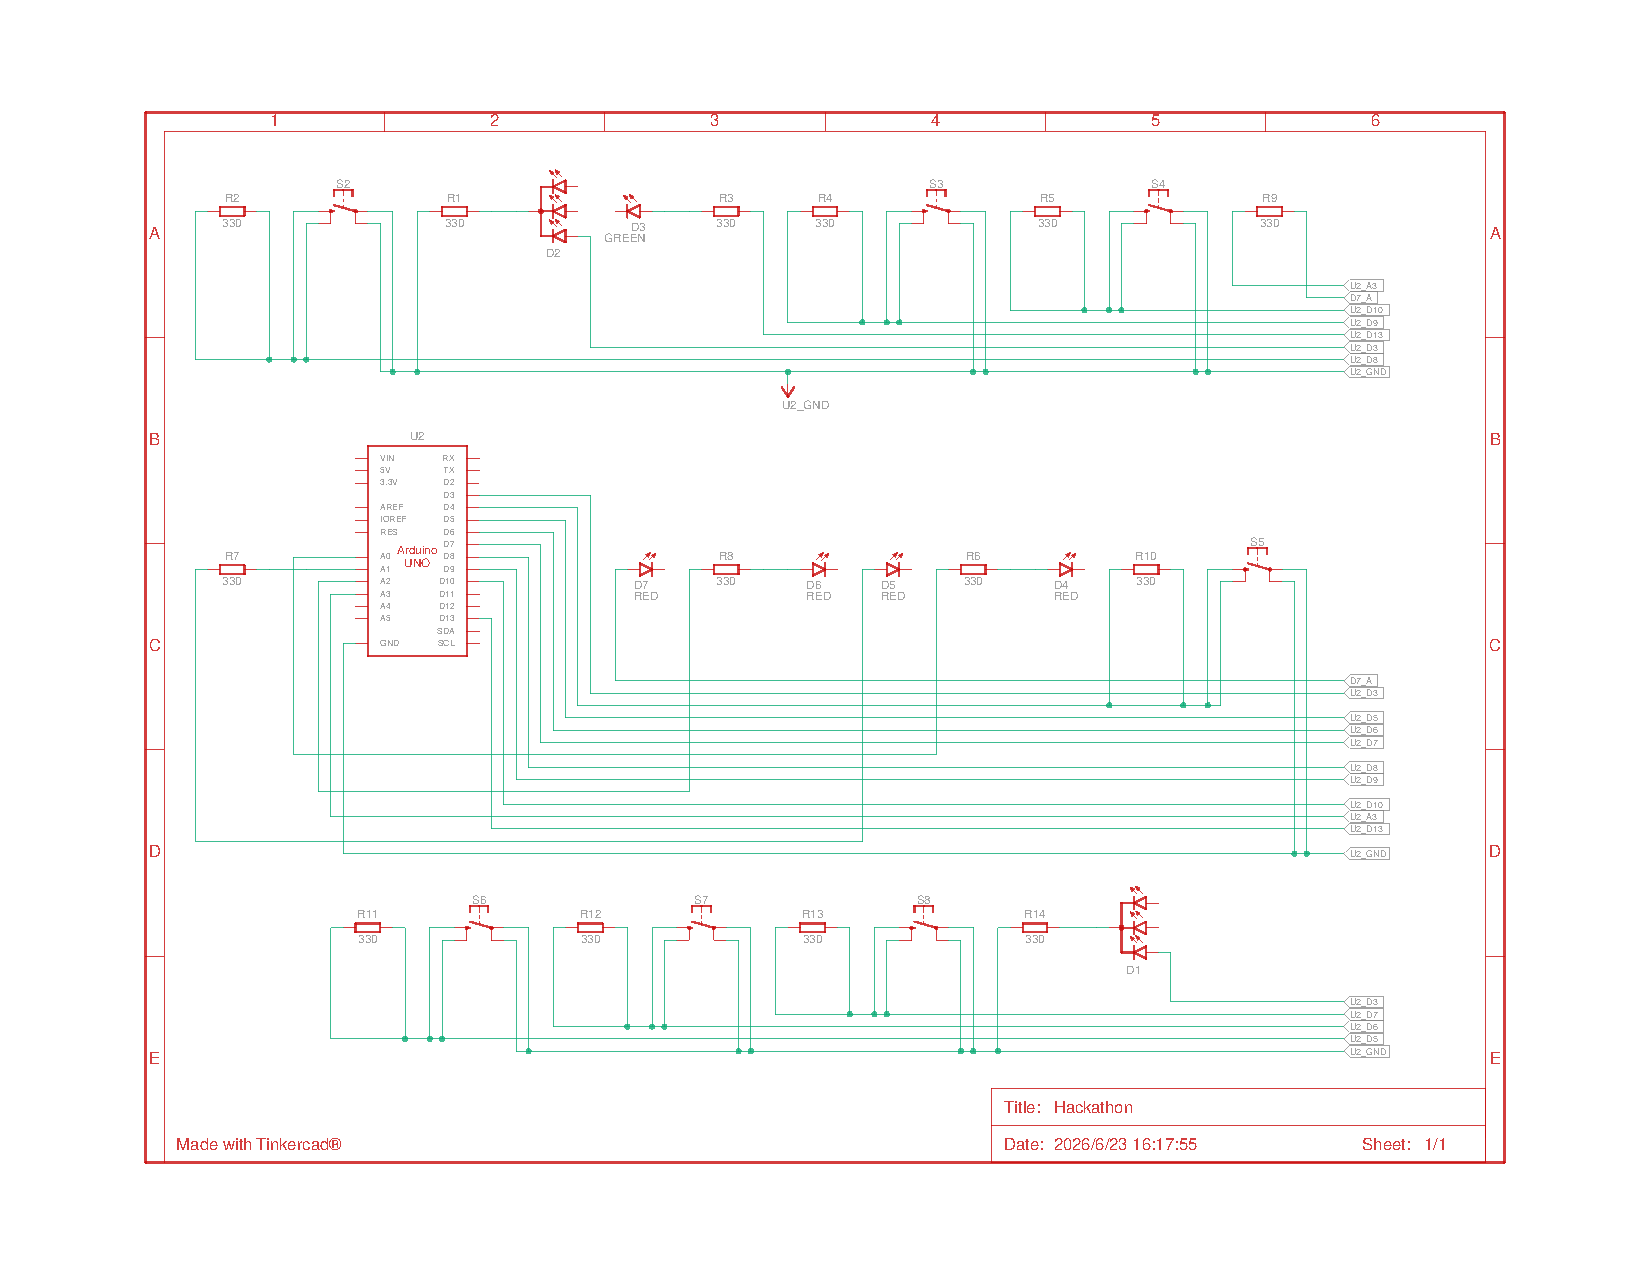
\includegraphics[width=0.95\textwidth]{circuit-diagram.pdf}
\caption{親機 hack-oya の回路図．D4--D7 子機ボタン群と D8 start ボタンを INPUT\_PULLUP で読み，A0--A3 の状態表示 LED を Arduino 側から駆動して点灯/消灯をトグル制御する．}
\label{fig:oya-schematic}
\end{figure}

\subsubsection{親機 hack-oya の回路実装イメージ}\label{sec:oya-photo}

図~\ref{fig:oya-photo} にブレッドボード上の実装イメージを示す．ボタンとボタンの隣接位置に状態表示 LED を物理的に配置することで，演奏者がどの子機を予約/参加させたかを目視で把握できる構成になっている．

\begin{figure}[H]
\centering
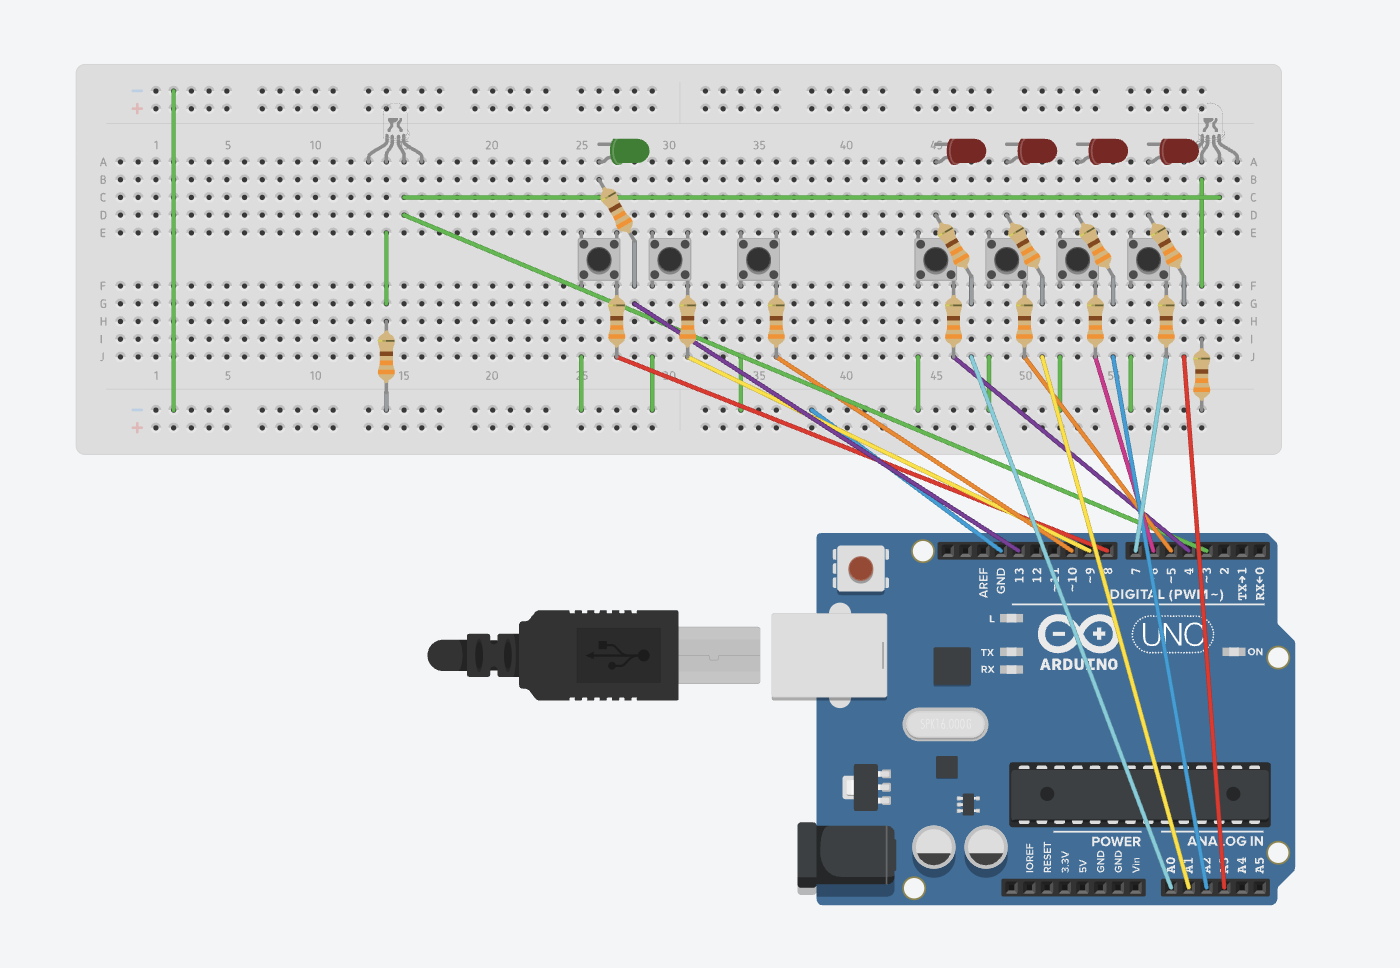
\includegraphics[width=0.95\textwidth]{image.png}
\caption{親機 hack-oya のブレッドボード実装イメージ．子機ボタン D4--D7 と隣接する A0--A3 トグル LED，start ボタン D8，IR LED（D3 駆動），動作確認用インジケータ LED（D13）が一枚のブレッドボードに収まる．}
\label{fig:oya-photo}
\end{figure}

\end{document}
